\begin{problem}[Munkres \S52, Ex.\,2]
Let $\alpha$ be a path in $X$ from $x_0$ to $x_1$; let $\beta$ be
a path in $X$ from $x_1$ to $x_2$. Show that if
$\gamma=\alpha*\beta$, then $\hat\gamma=\hat\beta\circ\hat\alpha$.
\end{problem}
\begin{proof}
By Theorem 52.1, the paths $\alpha$ and $\beta$ induce a group homomorphism
$\hat\alpha\colon\pi_1(X,x_0)\to\pi_1(X,x_1)$ and
$\hat\beta\colon\pi_1(X,x_1)\to\pi_1(X,x_2)$, respectively. We want to
show therefore that the induced homomorphism
$\hat\gamma=\widehat{\alpha*\beta}$ is in fact equivalent to the
composition $\hat\beta\circ\hat\alpha$. Let $[f]$ be a loop based at $x_0$
then
\begin{align*}
\hat\gamma([f])&=\widehat{\alpha*\beta}([f])\\
               &=\bigl[\,\overline{\alpha*\beta}\,\bigr]*[f]*[\alpha*\beta]\\
               &=\bigl[\bar\beta*\bar\alpha\bigr]*[f]*[\alpha]*[\beta]\\
\shortintertext{by the well-definedness of the path product operation, we have}
               &=[\bar\beta]*[\bar\alpha]*[f]*[\alpha]*[\beta]\\
\shortintertext{by associativity of the path product,}
               &=[\bar\beta]*([\bar\alpha]*[f]*[\alpha])*[\beta]\\
               &=[\bar\beta]*\hat\alpha([f])*[\beta]\\
\shortintertext{where $\alpha([f])$ is a loop based at $x_1$ so}
               &=\hat\beta\left(\hat\alpha([f])\right)\\
               &=\bigl(\hat\beta\circ\hat\alpha\bigr)([f]).
\end{align*}
Thus, the following diagram commutes
\begin{center}
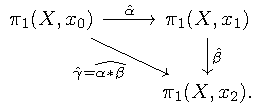
\includegraphics{figures/hw-10-pi-1-path-diagram}
\end{center}
\end{proof}
\newpage
\begin{problem}[Munkres \S52, Ex.\,3]
Let $x_0$ and $x_1$ be points of the path-connected space
$X$. Show that $\pi_1(X,x_0)$ is Abelian if and only if for every
pair $\alpha$ and $\beta$ of paths from $x_0$ to $x_1$, we have
$\hat\alpha=\hat\beta$.
\end{problem}
\begin{proof}
$\implies$ Suppose that $\pi_1(X,x_0)$ is Abelian. Then for any class of
loops about $x_0$, say $[f]$ and $[g]$, the product $[f]*[g]=[g]*[f]$. Let
$\alpha$ and $\beta$ be paths from $x_0$ to $x_1$. Then the induced map on
fundamental groups $\hat\alpha$ and $\hat\beta$ yield isomorphism by
Theorem 52.1 so that the map $\hat{\bar\beta}\circ\hat\alpha$ is an
automorphism of $\pi_1(X,x_0)$. Moreover, we have
\begin{align*}
\hat{\bar{\beta}}\circ\hat\alpha([f])
&=
\hat{\bar{\beta}}\bigl(\hat\alpha([f])\bigr)\\
&=
\hat{\bar{\beta}}\bigl([\bar\alpha]*[f]*[\alpha]\bigr)\\
&=
[\beta]*\bigl([\bar\alpha]*[f]*[\alpha]\bigr)*[\bar\beta]\\
\shortintertext{by associativity of the path product, we may rewrite the
  above expression as}
&=([\beta]*[\bar\alpha])*[f]*([\alpha]*[\bar\beta])
\shortintertext{noting that $[\beta]*[\bar\alpha]$ and
  $[\alpha]*[\bar\beta]$ are loops based at $x_0$, since $\pi_1(X,x_0)$ is
  Abelian, we have}
&=([\beta]*[\bar\alpha])*([\alpha]*[\bar\beta])*[f]\\
&=[e_{x_0}]*[f]\\
&=[f].
\end{align*}
Thus, $\hat{\bar{\beta}}\circ\hat\alpha=\id_{\pi_1(X,x_0)}$, i.e.,
$\hat\alpha=\hat\beta$.

$\impliedby$ Let $f$ and $g$ be loops about $x_0$. Then, since $X$ is path
connected, we claim that $f$ and $g$ are homotopic to the path product
$\alpha_1*\bar\beta_1$ and $\alpha_2*\bar\beta_2$ where $\alpha_i,\beta_i$
are paths from $x_0$ to $x_1$. More precisely, split $f$ into the paths
$f_1=f(t/2)$ and $f_2=f((t+1)/2)$; it is clear that $f=f_1*f_2$. Let
$x_2\coloneqq f_1(1)$ then there exists a path $\alpha$ from $x_2$ to $x_1$
since $X$ is path connected. Now we claim that the following
\[
H(x,t)\coloneqq f_1(x)*\alpha(tx)*\bar\alpha((1-t)x)*f_2(x)
\]
is a homotopy from $f=f_1*f_2$ to the extended loop $\tilde
f=f_1*\alpha*\bar\alpha*f_2$.
\begin{proof}[Proof of claim]
\renewcommand{\qedsymbol}{$\clubsuit$}
It is clear that $H$ is continuous since it is
a path products and multiplication on the unit interval $I$ is
continuous so $tx$ is continuous. Lastly,
$H(x,0)=f_1(x)*\alpha(0)*\bar\alpha(0)*f_2(x)$ and
$H(x,1)=f_1(x)*\alpha(x)*\bar\alpha(x)*f_2(x)$.
\end{proof}
Now, let $f\simeq_p\alpha_1*\bar\beta_1$ and
$g\simeq_p\alpha_2*\bar\beta_2$ where $\alpha_i,\beta_i$ are
paths from $x_0$ to $x_1$. Then we have
\begingroup
\allowdisplaybreaks
\begin{align*}
[f]*[g]*[\bar f]*[\bar g]
&=
[\alpha_1*\bar\beta_1]*[\alpha_2*\bar\beta_2]*
\bigl[\overline{\alpha_1*\bar\beta_1}\bigr]*
\bigl[\overline{\alpha_2*\bar\beta_2}\bigr]\\
&=
[\alpha_1*\bar\beta_1]*[\alpha_2*\bar\beta_2]*
[\beta_1*\bar\alpha_1]*[\beta_2*\bar\alpha_2]\\
&=
[\alpha_1]*[\bar\beta_1]*[\alpha_2]*[\bar\beta_2]*
[\beta_1]*[\bar\alpha_1]*[\beta_2]*[\bar\alpha_2]\\
&=\hat{\bar{\alpha}}_1\bigl([\bar\beta_1]*[\alpha_2]*[\bar\beta_2]*[\beta_1]\bigr)*[\beta_2]*[\alpha_2]\\
&=\hat{\bar{\alpha}}_1\bigl(\hat\beta_2([\alpha_2]*[\bar\beta_2])\bigr)*[\beta_2]*[\bar\alpha_2]\\
&=[\alpha_2]*[\bar\beta_2]*[\beta_2]*[\bar\alpha_2]\\
&=[\alpha_2]*[e_{x_0}]*[\bar\alpha_2]\\
&=[\alpha_2]*[\bar\alpha_2]\\
&=[e_{x_0}].
\end{align*}
\endgroup
Thus, $\pi_1(X,x_0)$ is Abelian.
\end{proof}
\newpage
\begin{problem}[Munkres \S52, Ex.\,4]
Let $A\subset X$; suppose $r\colon X\to A$ is continuous map such
that $r(a)=a$ for each $a\in A$. (The map $r$ is called a
\emph{retraction} of $X$ onto $A$.) If $a_0\in A$, show that
\[
r_*\colon\pi_1(X,x_0)\longrightarrow\pi_1(A,a_0)
\]
is surjective.
\end{problem}
\begin{proof}
Suppose $f$ is a loop in $A$ based at $a$. Then, extending the
codomain of $f$ to $X$, $f$ is a loop in $X$ based at $a$. Then,
since $r(a)=a$ for all $a$ and $f(I)\subset A$,
$r_*([f])=[p(f)]=[f]$ so $r_*$ is surjective.
\end{proof}
\newpage
\begin{problem}[Munkres \S53, Ex.\,6]
Show that if $X$ is path connected, the homomorphism induced by a
continuous map is independent of the base point, up to
isomorphisms of the groups involved. More precisely, let $h\colon
X\to Y$ be continuous, with $h(x_0)=y_0$ and $h(x_1)=y_1$. Let
$\alpha$ be a path in $X$ from $x_0$ to $x_1$, and let
$\beta=h\circ\alpha$. Show that
\[
\hat\beta\circ(h_{x_0})_*=(h_{x_1})_*\circ\hat\alpha.
\]
This equation expresses the fact that the following diagram of
maps ``commutes''
\begin{center}
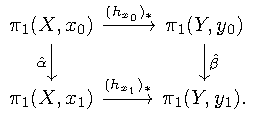
\includegraphics{figures/hw-10-path-connected-hom-indep}
\end{center}
\end{problem}
\begin{proof}
Unpacking the expression on the left, we have the following
sequence of equalities: Let $f$ be a loop in $X$ based at $x_0$
then
\begin{align*}
\bigl(\hat\beta\circ(h_{x_0})_*\bigr)([f])
&=\hat\beta\bigl((h_{x_0})_*([f])\bigr)\\
&=\hat\beta\bigl([h(f)]\bigr)\\
&=[\bar\beta]*[h(f)]*[\beta]\\
&=\bigl[\,\overline{h\circ\alpha}\,\bigr]*[h(f)]*[h\circ\alpha]\\
&=[h\circ\bar\alpha]*[h(f)]*[h\circ\alpha]\\
\shortintertext{but since $(h_{x_1})_*$ is a homomorphism}
&=(h_{x_0})_*(\bar\alpha*f*\alpha)\\
&=(h_{x_1})_*\bigl(\hat\alpha([f])\bigr)\\
&=\bigl((h_{x_1})_*\circ\hat\alpha\bigr)([f]).
\end{align*}
\end{proof}
\newpage
\begin{problem}[Munkres \S55, Ex.\,1]
Show that if $A$ is a retract of $B^2$, then every continuous map
$f\colon A\to A$ has a fixed point.
\end{problem}
\begin{proof}
Suppose that $A$ is a retract of $B^2$. Let $r\colon B^2\to A$ one such
retraction. If $f\colon A\to A$ is a continuous map, then $f\circ r$ is a
continuous map, by Theorem 18.2(c), from $B^2$ to $A$. Expanding the
codomain of $f$ to $B^2$, i.e., composing with the canonical injection
$\iota\colon A\hookrightarrow B^2$, we have a continuous mapping
$\tilde{f}\colon B^2\to B^2$ that coincides with $f$ in $A$. Then, by
Theorem 55.6, $\tilde f$ has a fixed point, i.e., $\tilde{f}(x)=x$ for some
$x\in B^2$. By the Brouwer fixed-point theorem for the disc, there exists a
point $x\in B^2$ such that $\tilde{f}(x)=x$, but $\im{\tilde{f}}=\im
f\subset A$ so $x\in A$. It follows that $f$ has a fixed point.
\end{proof}
\newpage
\begin{problem}[Munkres \S55, Ex.\,2]
Show that if $h\colon S^1\to S^1$ is nulhomotopic, then $h$ has a
fixed point and $h$ maps some point $x$ to its antipode $-x$.
\end{problem}
\begin{proof}
\end{proof}
\newpage
\begin{problem}[(A)]
Prove that every $m$-manifold is locally path-connected.
\end{problem}
\begin{proof}
Suppose $M$ is an $m$-manifold. Let $x\in M$ and $U'$ be an arbitrary
neighborhood of $x$. Then, since $M$ is a manifold, there exists an open
neighborhood $U$ of $x$ that is homeomorphic to an open subset, say $V$, of
$\RR^m$. Let $h\colon U\to V$ be a homeomorphism. Then $h(U\cap U')$ is
open in $U$ so by Theorem 16.2, $h(U\cap U')$ is open in
$\RR^m$. Therefore, for sufficiently small values of $\delta>0$, we have
the inclusion $B(h(x),\delta)\subset h(U\cap U')$. We claim that
$W\coloneqq h^{-1}(B(h(x),\delta))$ is a path-connected neighborhood of $x$
contained in $U'$.

Containment is clear for $h$ is a bijection and we have that $W\subset
U\cap U'\subset U'$. By Example 3 in Munkres \S24 we know that open balls
in $\RR^m$ are path-connected therefore given $y_0=h(x_0),y_1=h(x_1)\in
h(W)$, there exists a path $p\colon I\to h(W)$ with $p(0)=y_0$ and
$p(1)=y_1$. Then $q\coloneqq \left(\bigl.(h^{-1})\bigr|_{h(W)}\circ
  p\right)\colon I\to W$ is a path in $W$ from $x_0$ to $x_1$. It is clear
that $q$ is continuous by Theorem 18.2(c) since it is a composition of
continuous functions (where $\bigl.(h^{-1})\bigr|_{h(W)}$ is continuous by
Theorem 18.2(d) since it is the restriction of a continuous
function). Lastly, $q(0)=x_0$ and $q(1)=x_1$. Since $x_0$ and $x_1$ were
arbitrary, it follows that $W$ is path-connected. Therefore, $M$ is locally
path-connected.
\end{proof}
\newpage
\begin{problem}[(B)]
Prove that every $m$-manifold is regular.
\end{problem}
\begin{proof}
\end{proof}
\newpage
\begin{problem}[(C)]
Prove that there is no $1$-$1$ continuous function $\iota\colon
S^1\to\RR$. You may assume any fact about trigonometric
functions. (Note: this shows in particular that there is no
$\iota\colon S^1\to\RR$ with $p\circ\iota$ equal to the identity
map, where $p$ is the map in the note on the Fundamental Group of
the Circle.)
\end{problem}
\begin{proof}
\end{proof}
\newpage
\begin{problem}[(D)]
Prove Proposition C from the note on the Fundamental Group of the Circle.
\end{problem}
\begin{proof}
\end{proof}

%%% Local Variables:
%%% mode: latex
%%% TeX-master: "../MA571-HW-Current"
%%% End:
